For the tests the positions of beacons are fixed and the initial poses too.

\begin{figure}[H]
\centering
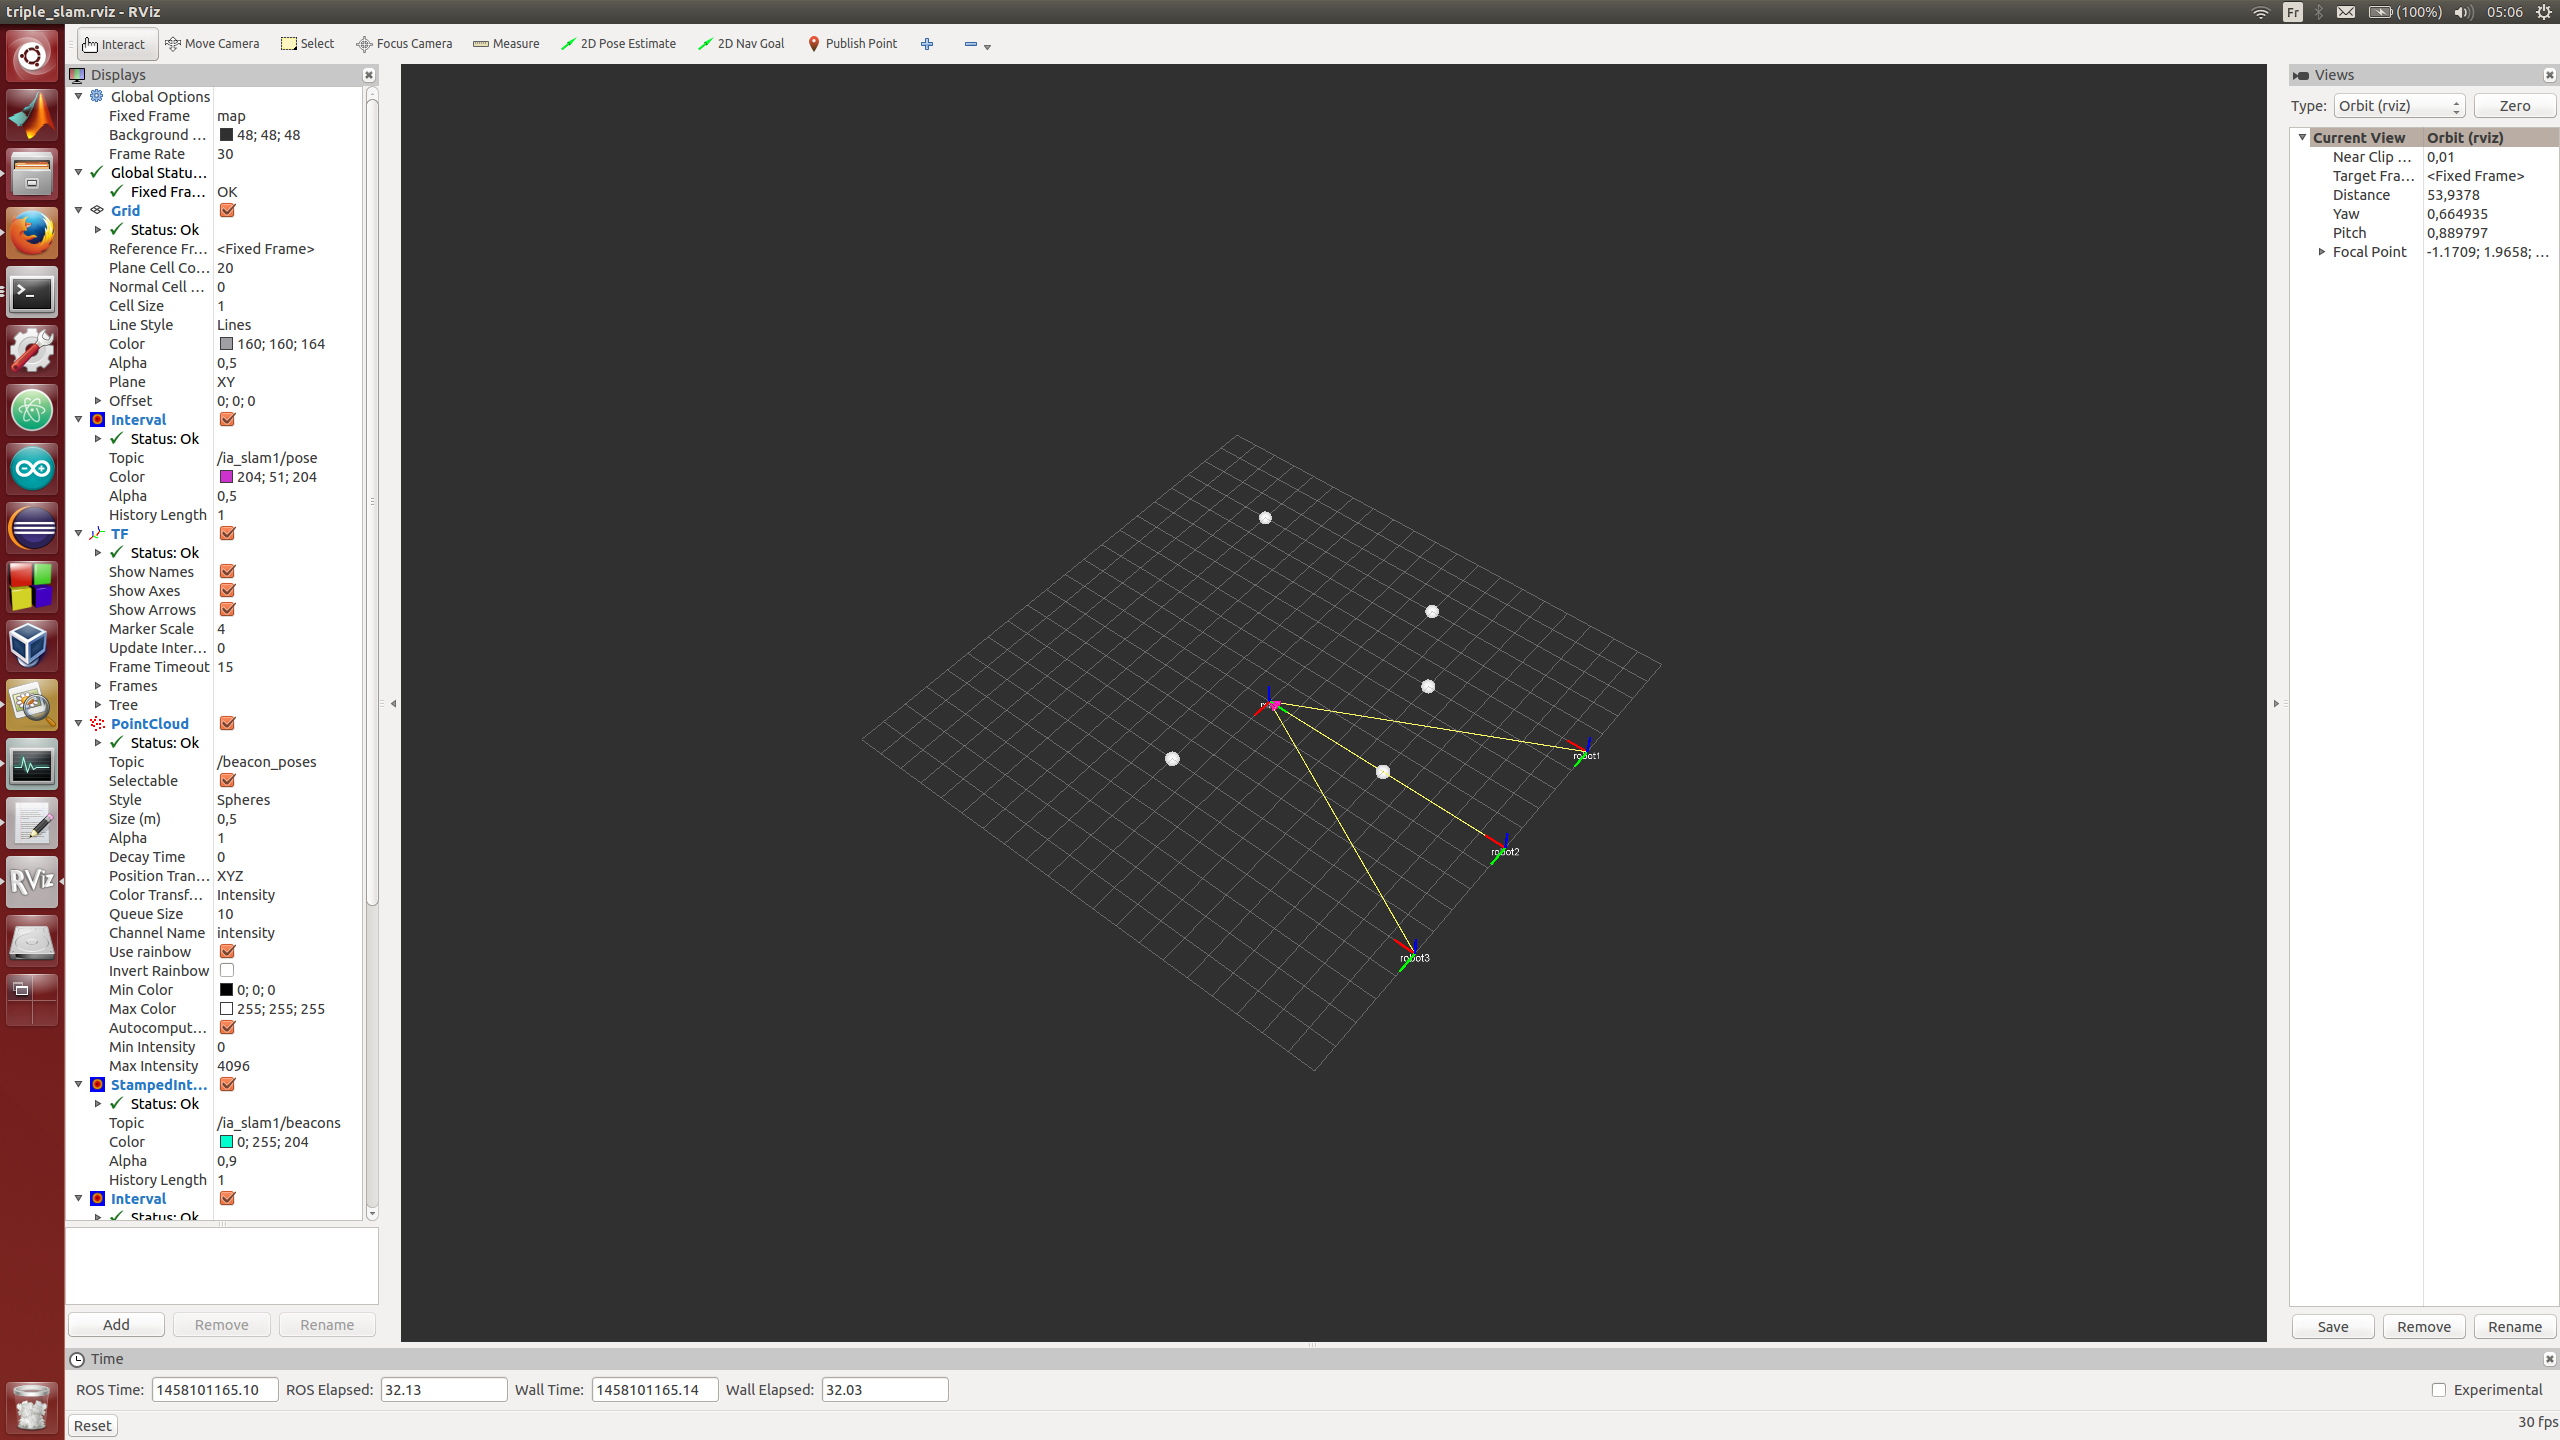
\includegraphics[trim={35cm 15cm 30cm 15cm},clip,scale=0.2,angle=0]{pose_initial.png}
\caption{Initial Poses of the robots.}
\label{fig:initialPose}
\end{figure}

\section{One Robot}

For the test, one robot is used with a sensor precision of 10cm  and a precision for the starting position of 10cm. A case is 1mx1m.

\begin{figure}[H]
\centering
\begin{minipage}[b]{0.4\textwidth}
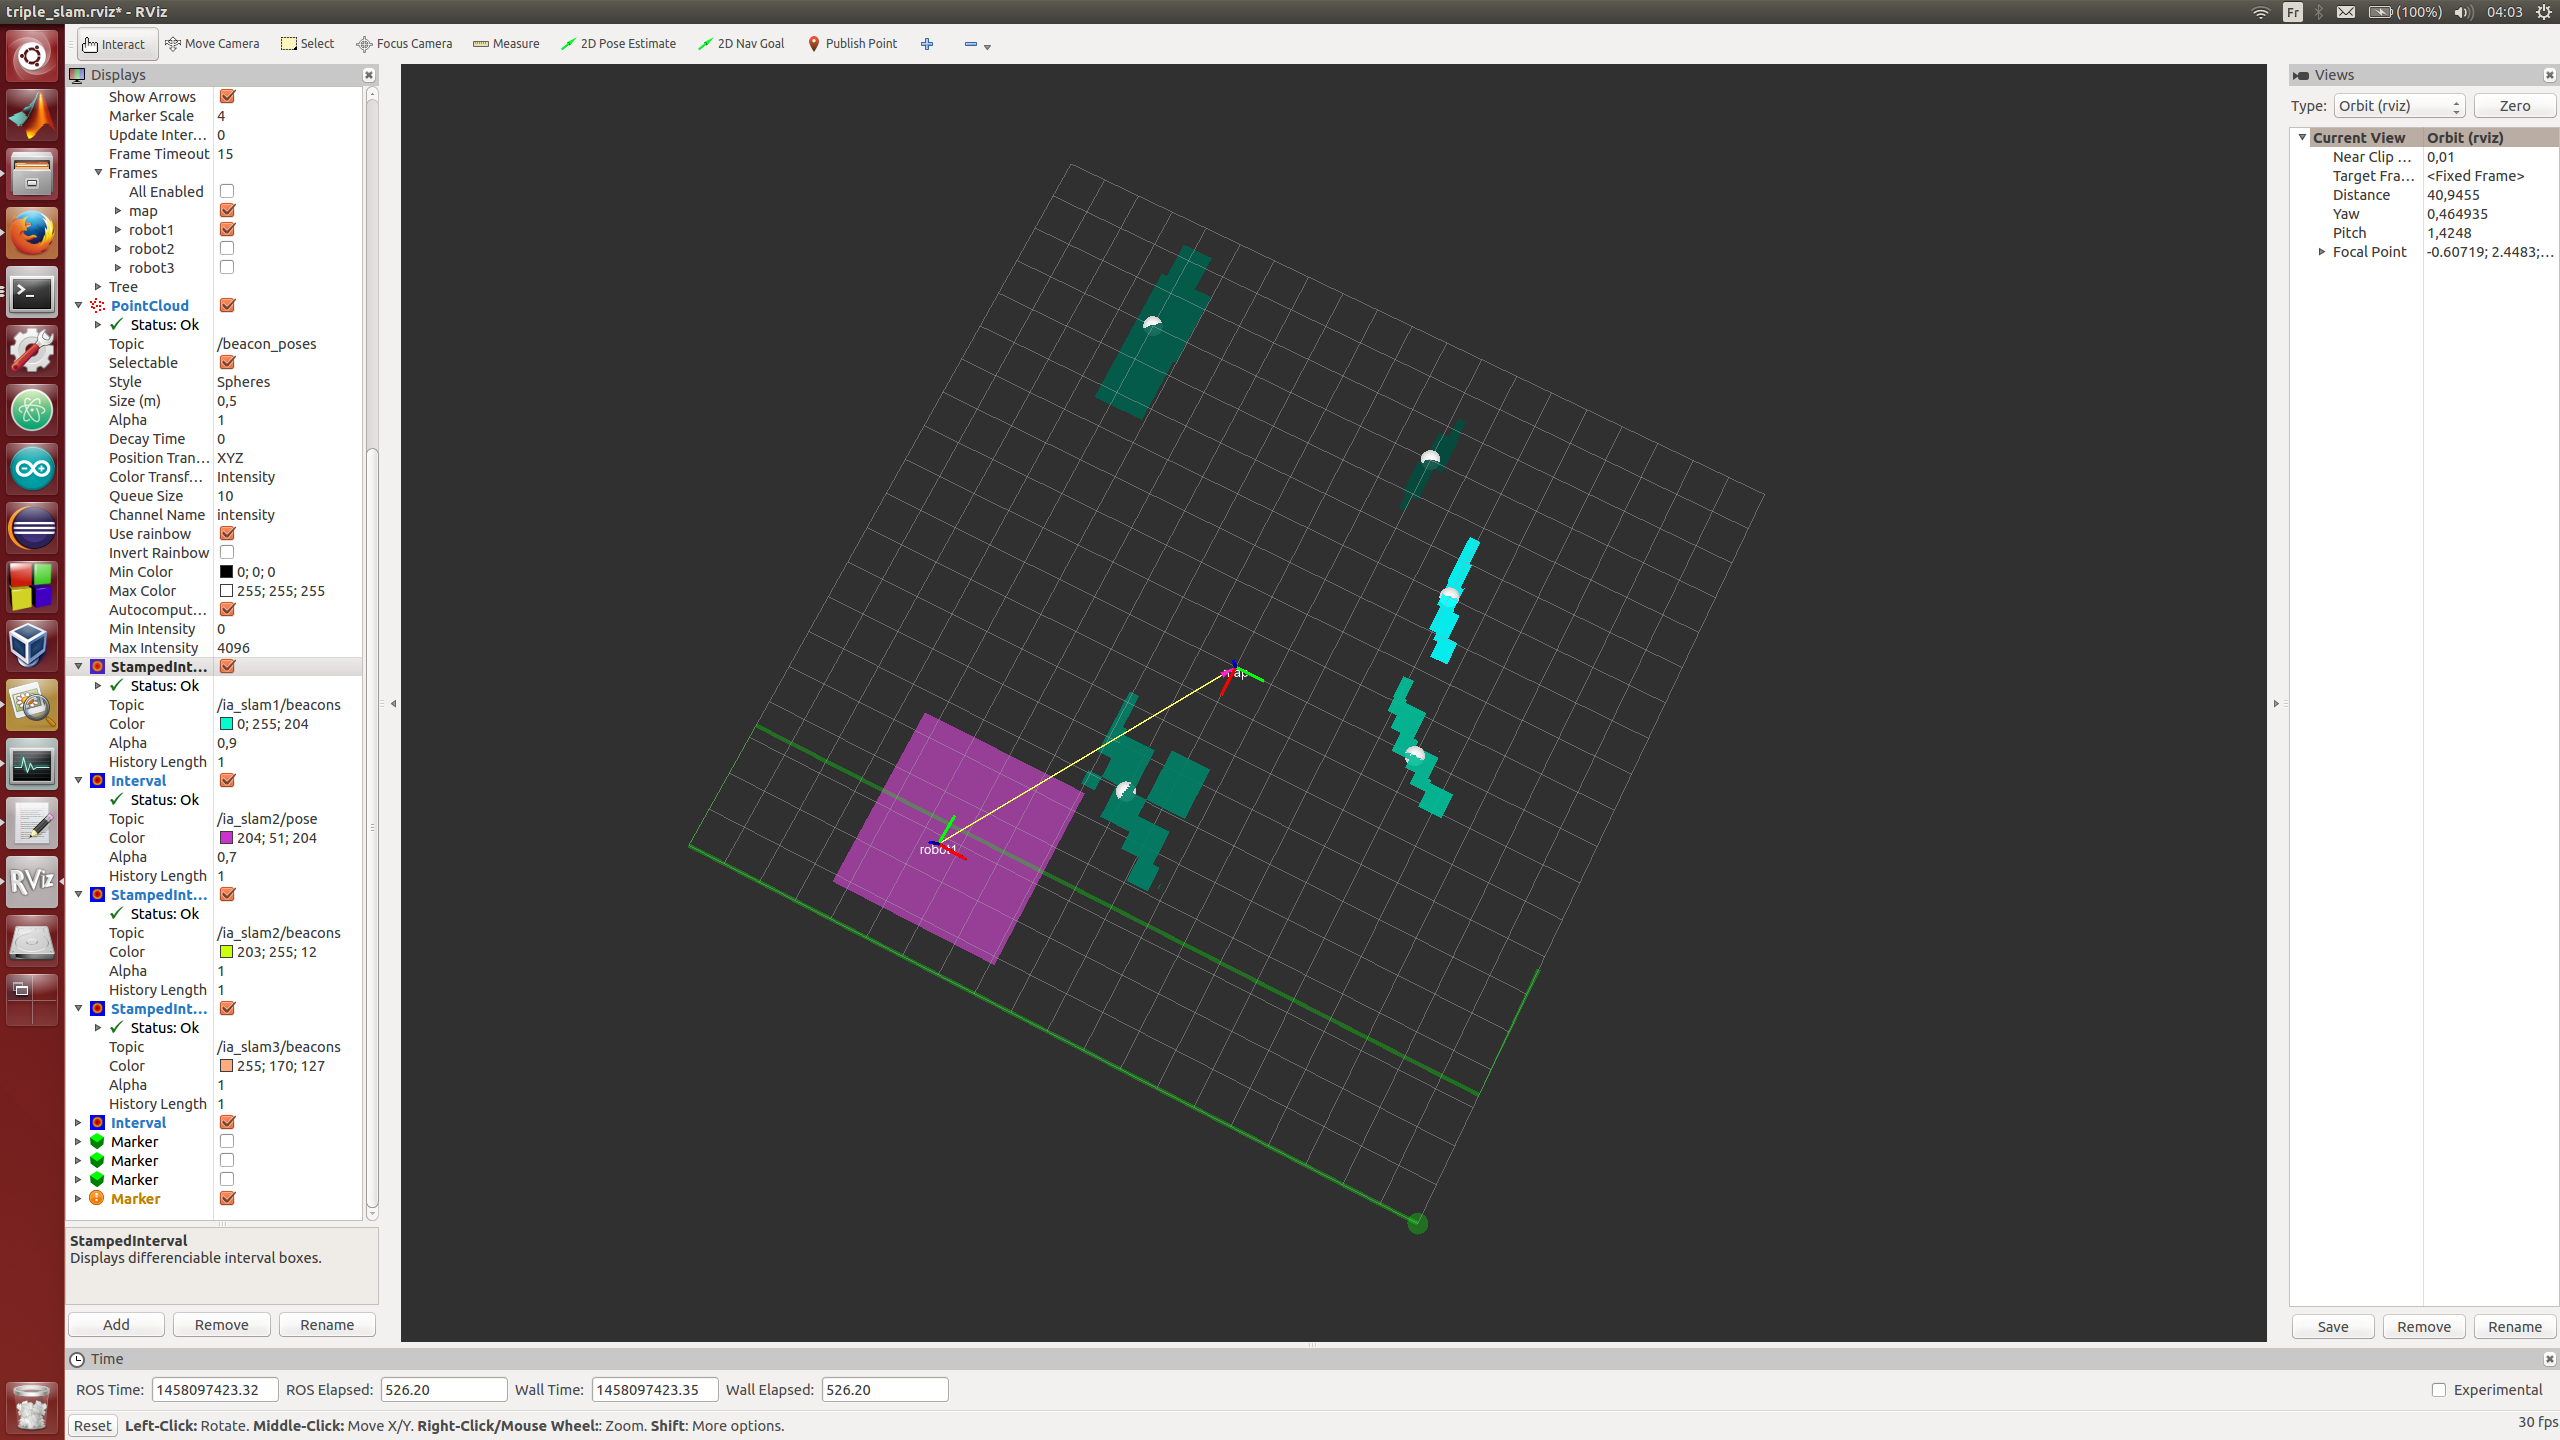
\includegraphics[trim={25cm 7cm 30cm 6cm},clip,scale=0.15,angle=0]{one_robot_result.png}
\caption{Visualization with one robot scanning the area (start).}
\label{fig:oneRobResDeb}
\end{minipage}
\begin{minipage}[b]{0.4\textwidth}
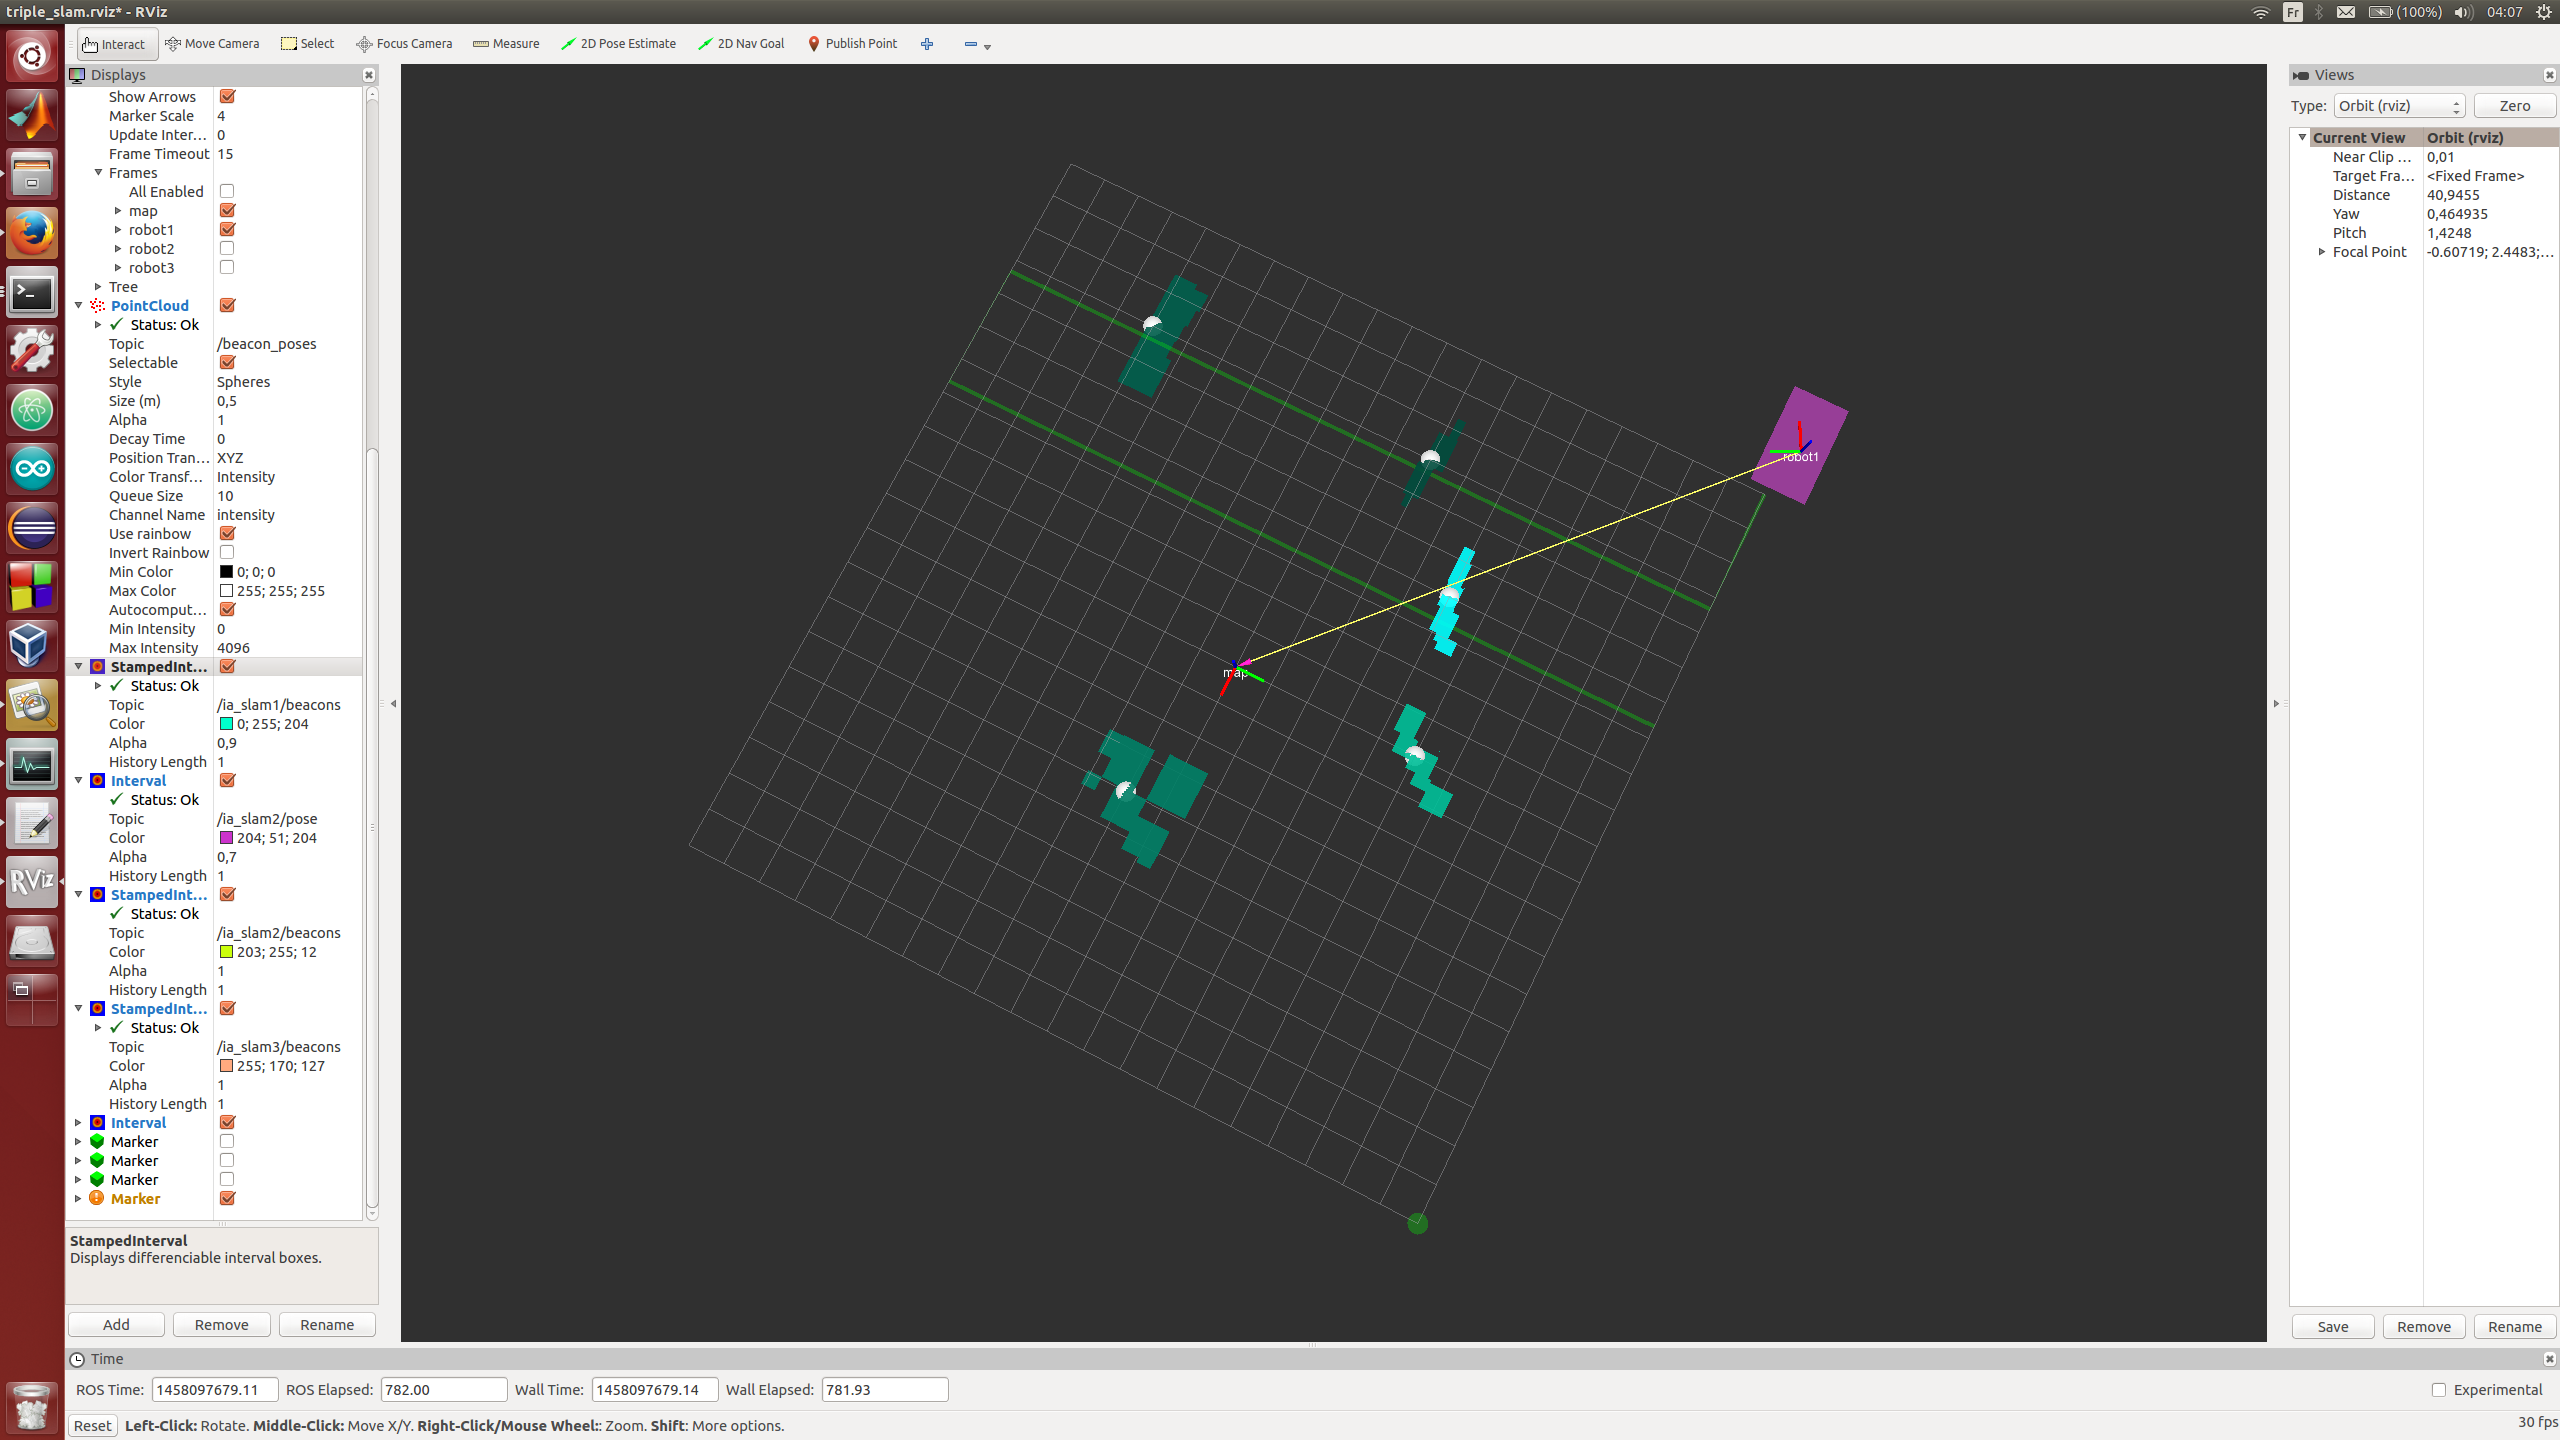
\includegraphics[trim={25cm 7cm 25cm 6cm},clip,scale=0.15,angle=0]{one_robot_result_end.png}
\caption{Visualization with one robot scanning the area (end).}
\label{fig:oneRobResEnd}
\end{minipage}
\end{figure}

The images~\ref{fig:oneRobResDeb} and~\ref{fig:oneRobResEnd} are obtained with the robot going directly to the scanning without doing the first pass (see subsection~\ref{ssec:pathgen}).

The estimate of the beacons has not got good quality the estimate for one beacon are spread out around it therefore the estimate of the robot  is not good and consequently the controller can't correctly handle the robot and in figure~\ref{fig:oneRobResDeb} the robot does not follow exactly the path (green line) and has an offset.

\section{Two Robots}

For this test, one robot is used with a sensor precision of 10cm  and a precision for the starting position of 70cm. In this test the second robot follows the same path as the first one.

\begin{figure}[H]
\centering
\begin{minipage}[b]{0.4\textwidth}
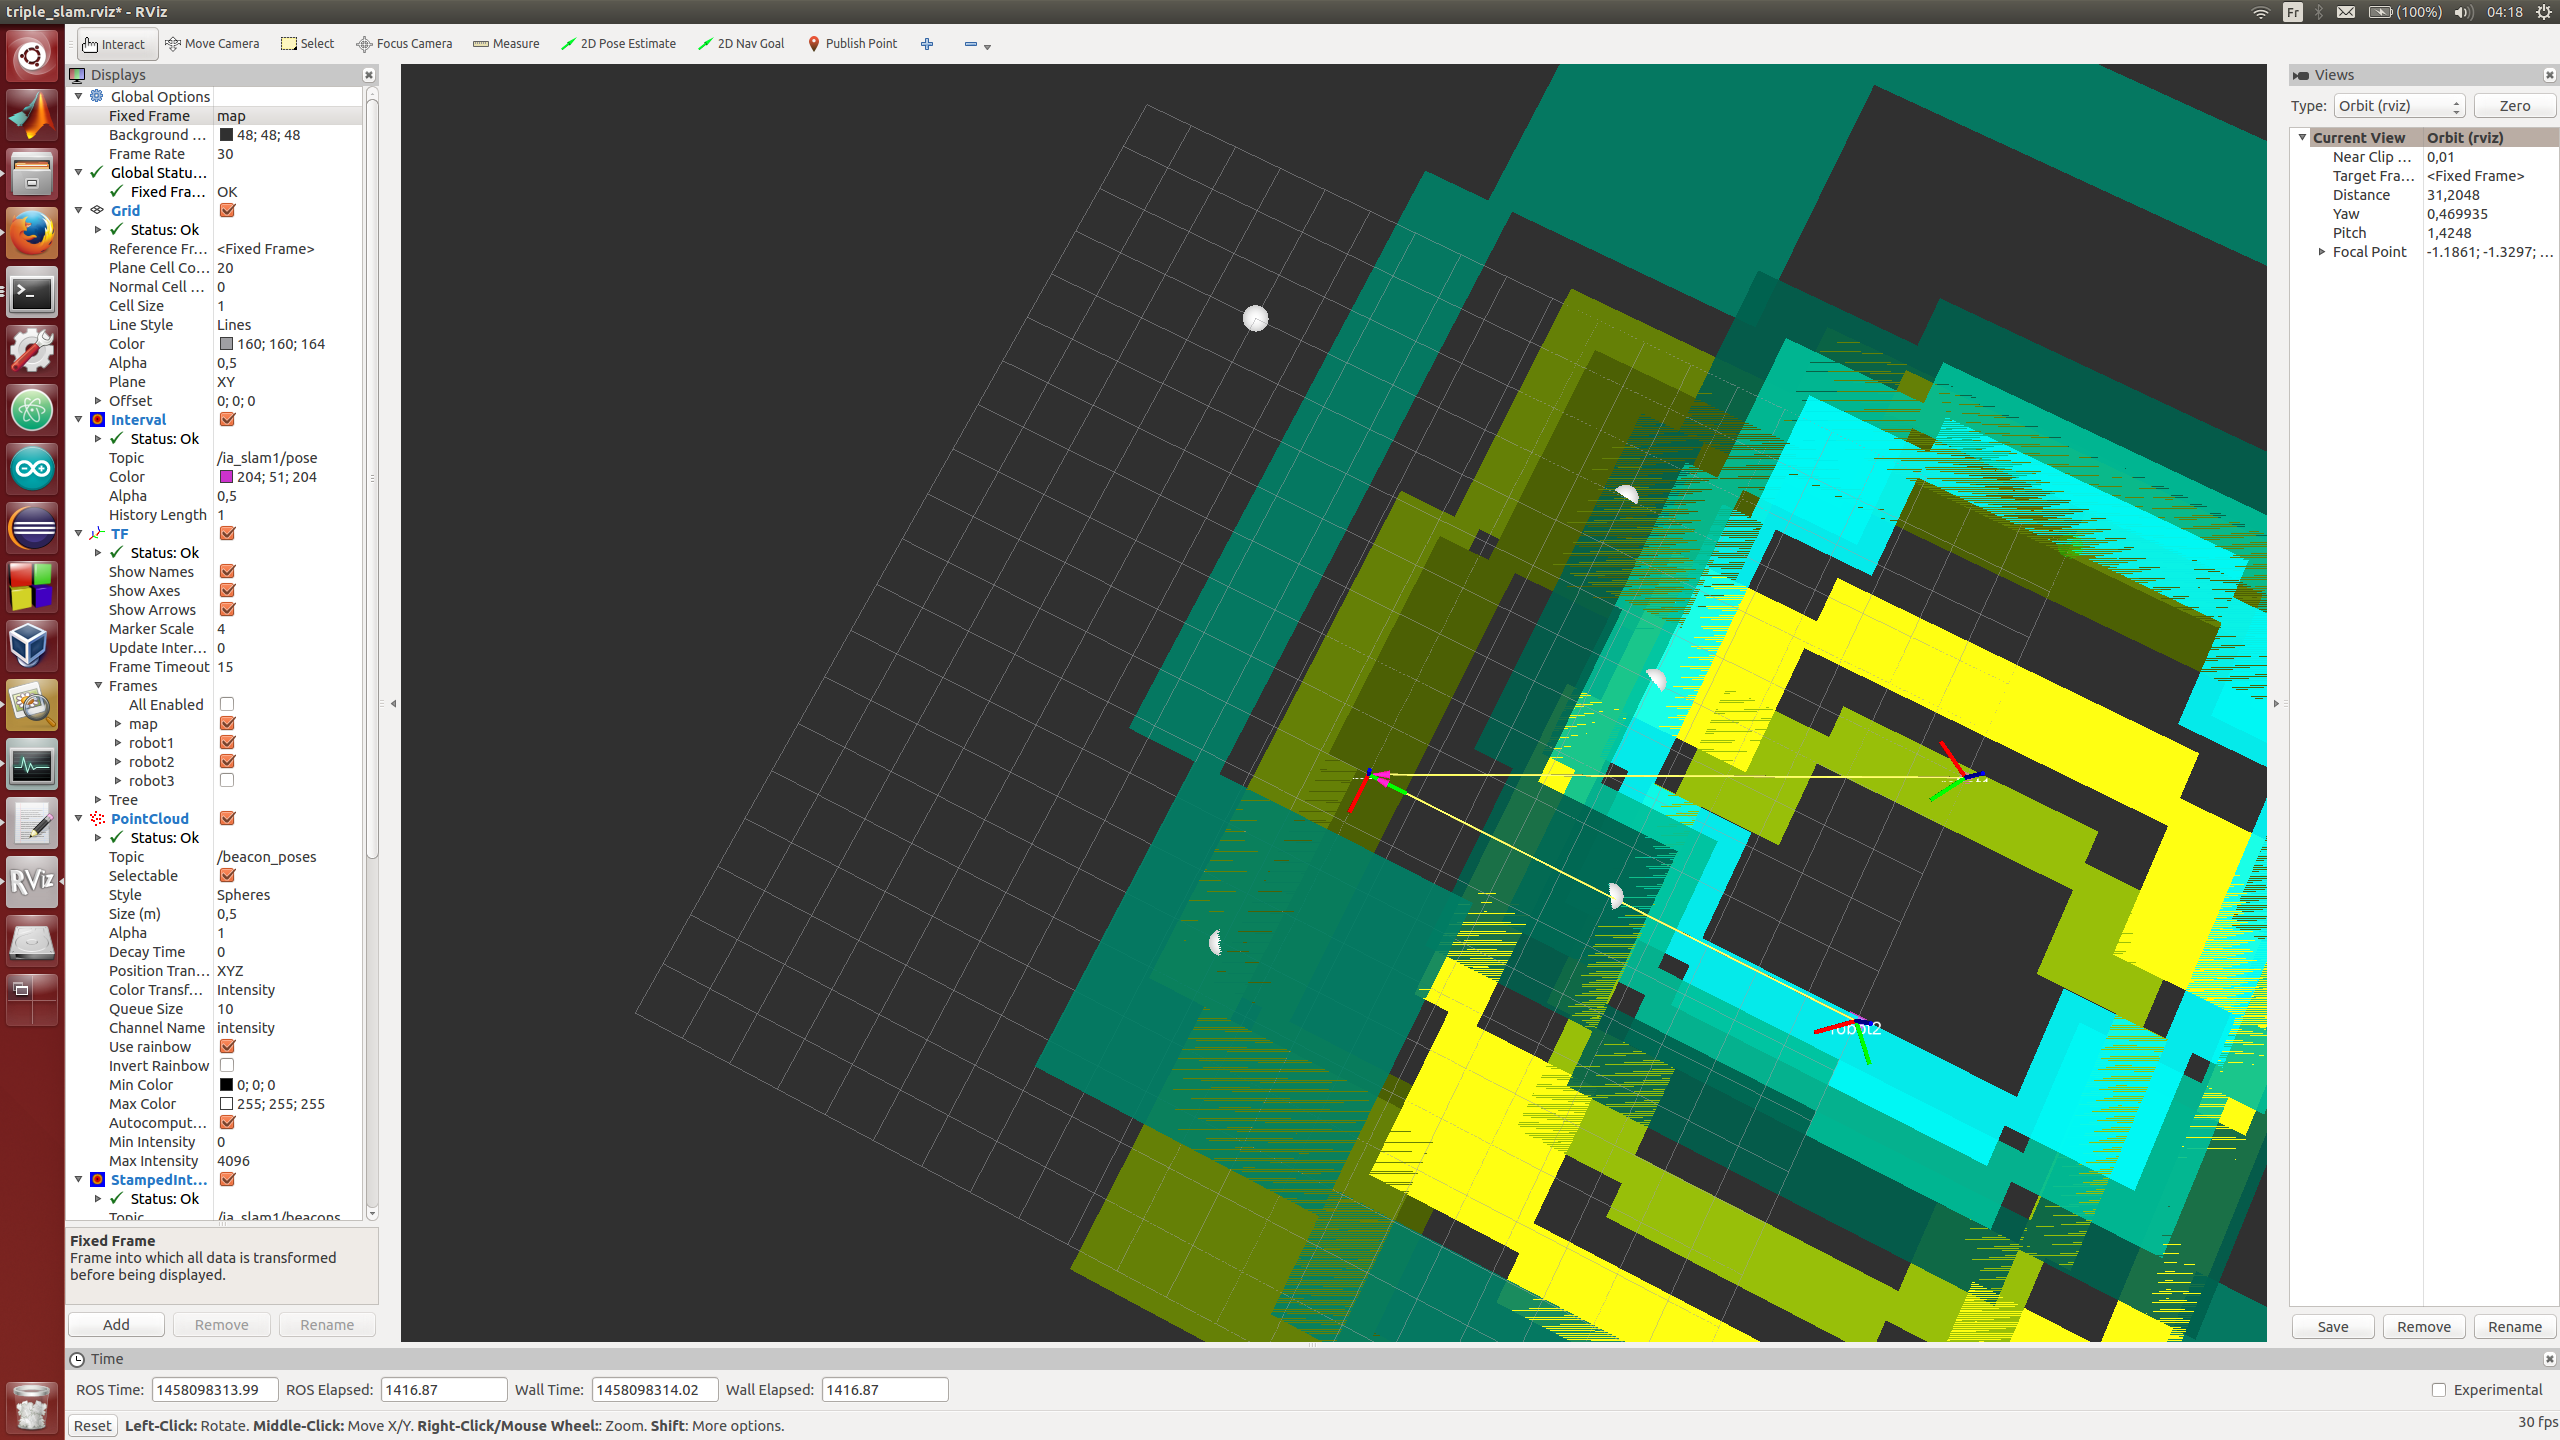
\includegraphics[trim={33cm 7cm 20cm 6cm},clip,scale=0.15,angle=0]{start_two.png}
\caption{Visualization of start of the slam without discussion between robots.}
\label{fig:twoRobResDeb}
\end{minipage}
\begin{minipage}[b]{0.4\textwidth}
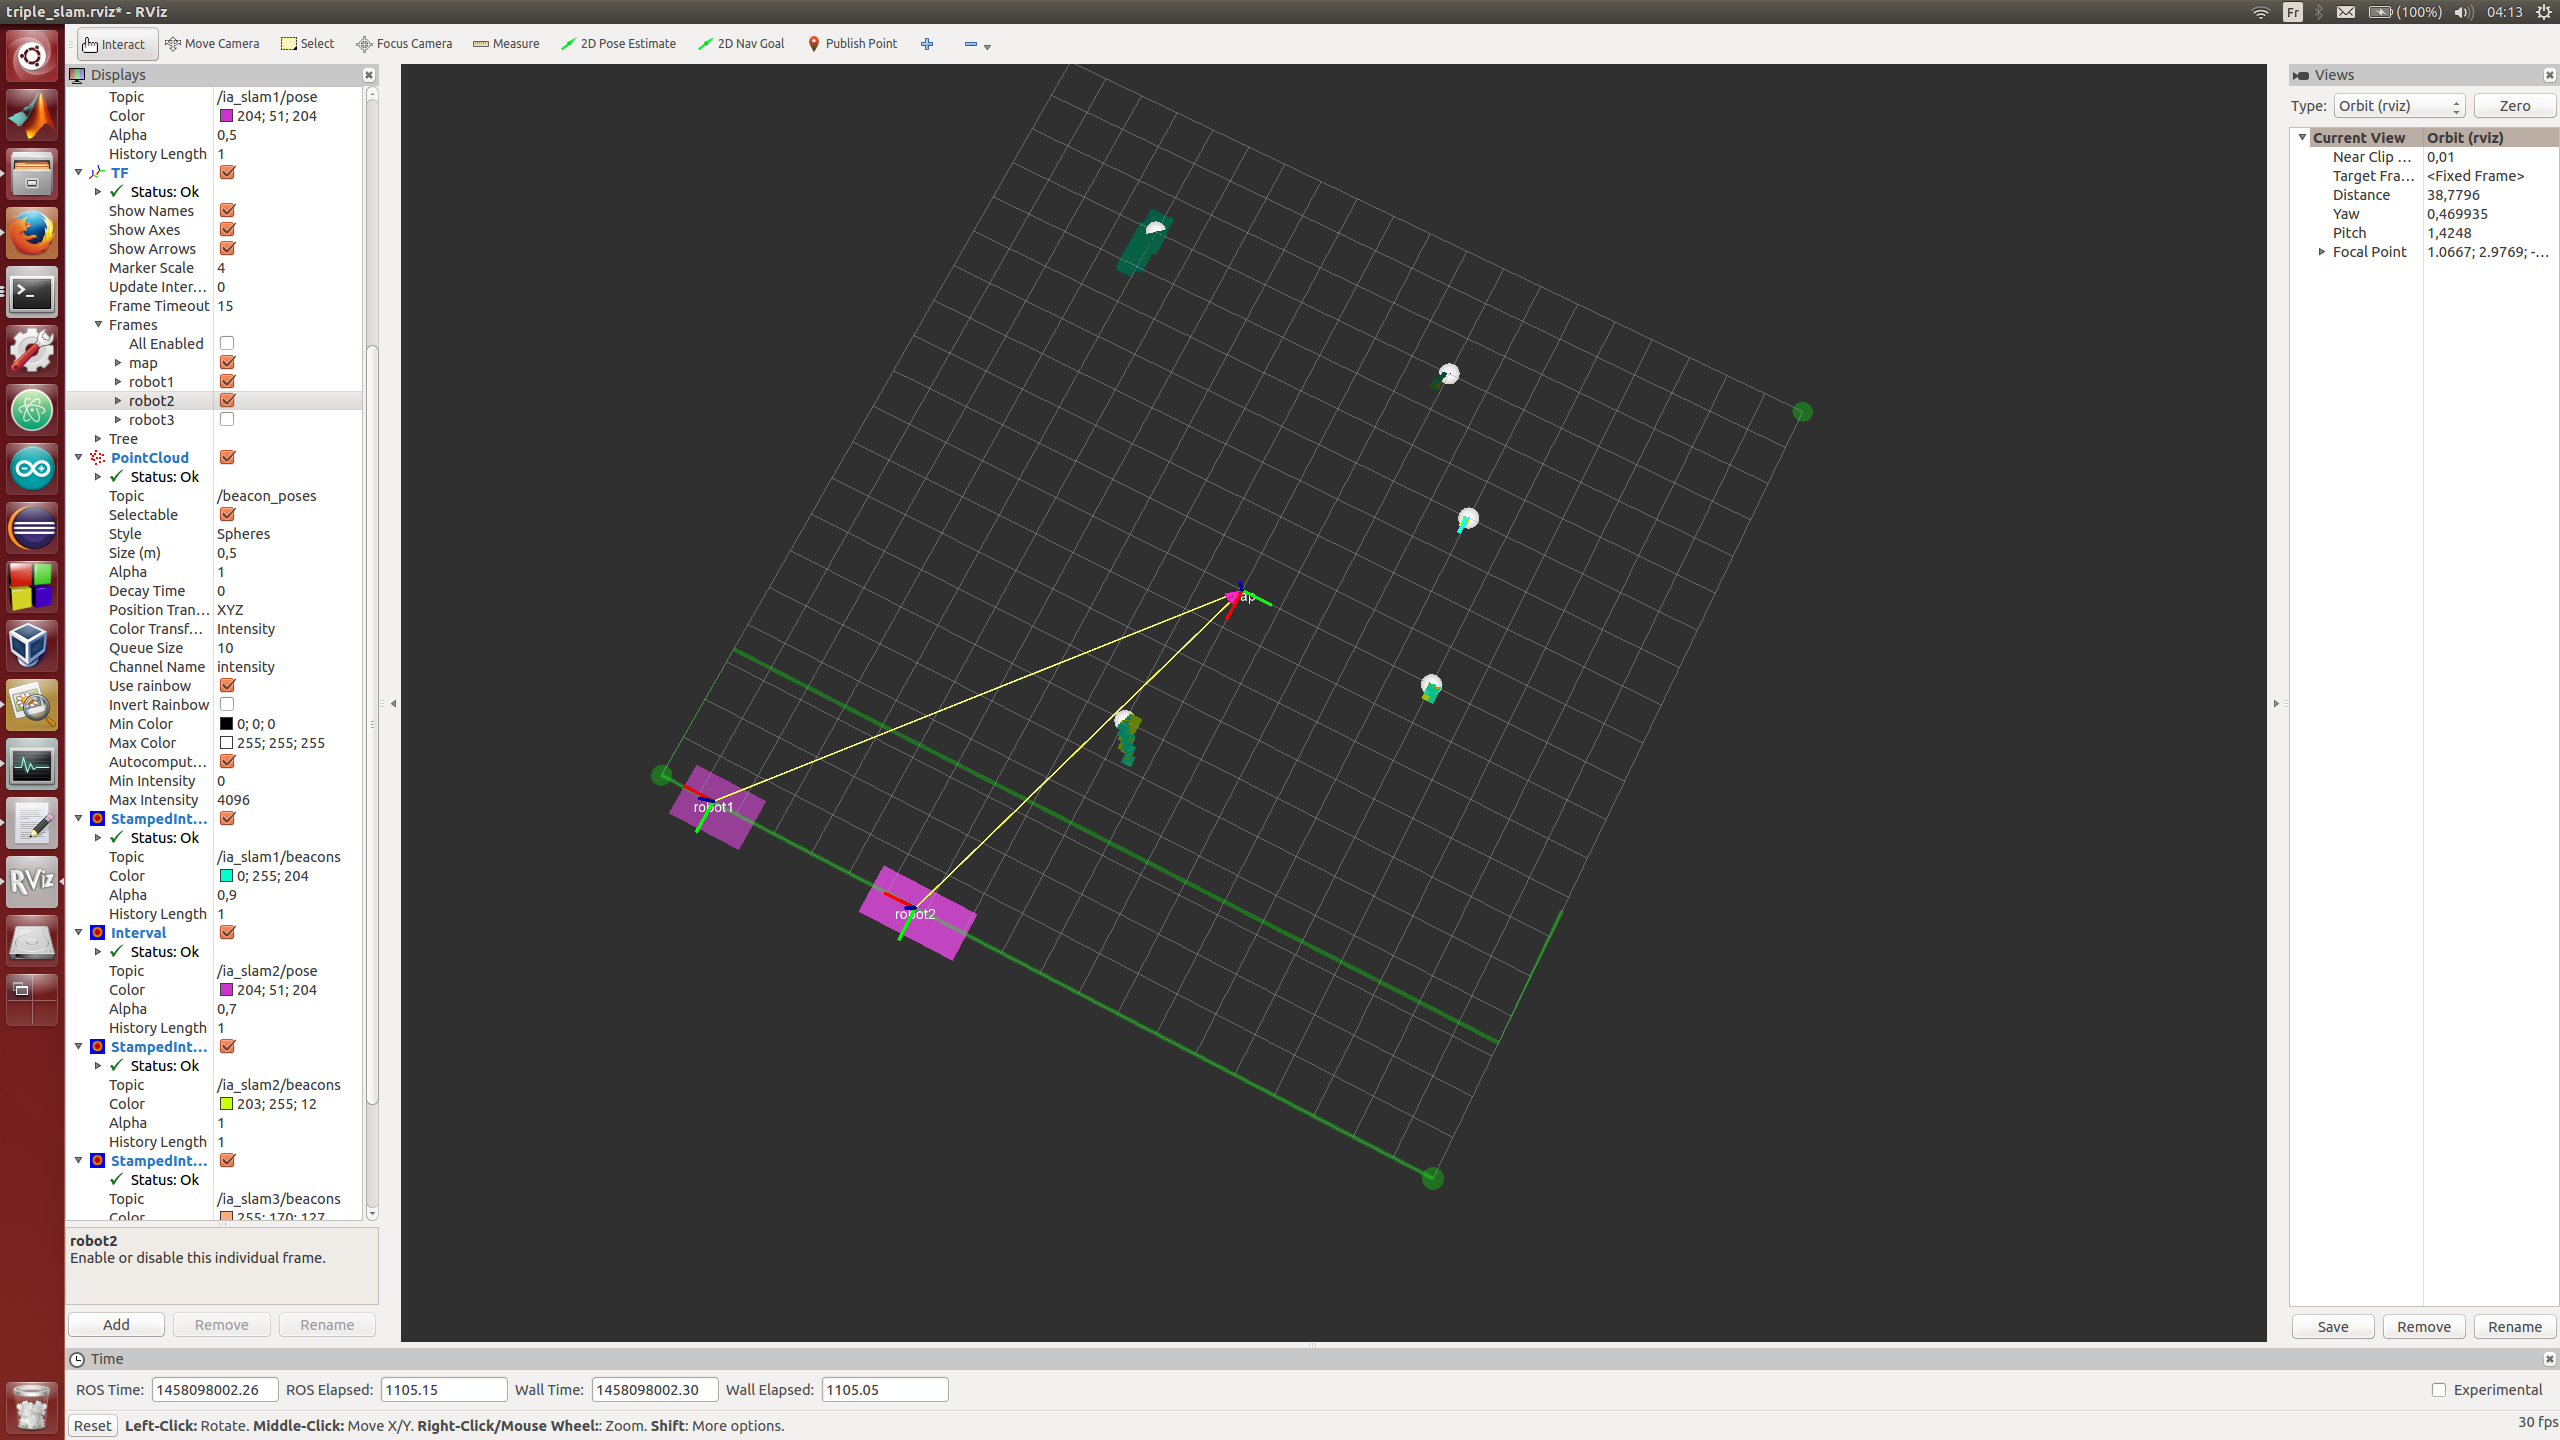
\includegraphics[trim={20cm 7cm 30cm 6cm},clip,scale=0.15,angle=0]{two_robot_start_scanning.png}
\caption{Visualization of the two robots following the scanning path.}
\label{fig:twoRobResEnd}
\end{minipage}
\end{figure}

With two robots communicating the estimations become more precise and allow a better path following(figure~\ref{fig:twoRobResEnd}.
From them the it could continue to more robots but some errors have happened. Indeed sometime the estimation for a beacon is wrong, the boxes do not include the beacon. 

\begin{figure}[H]
\centering
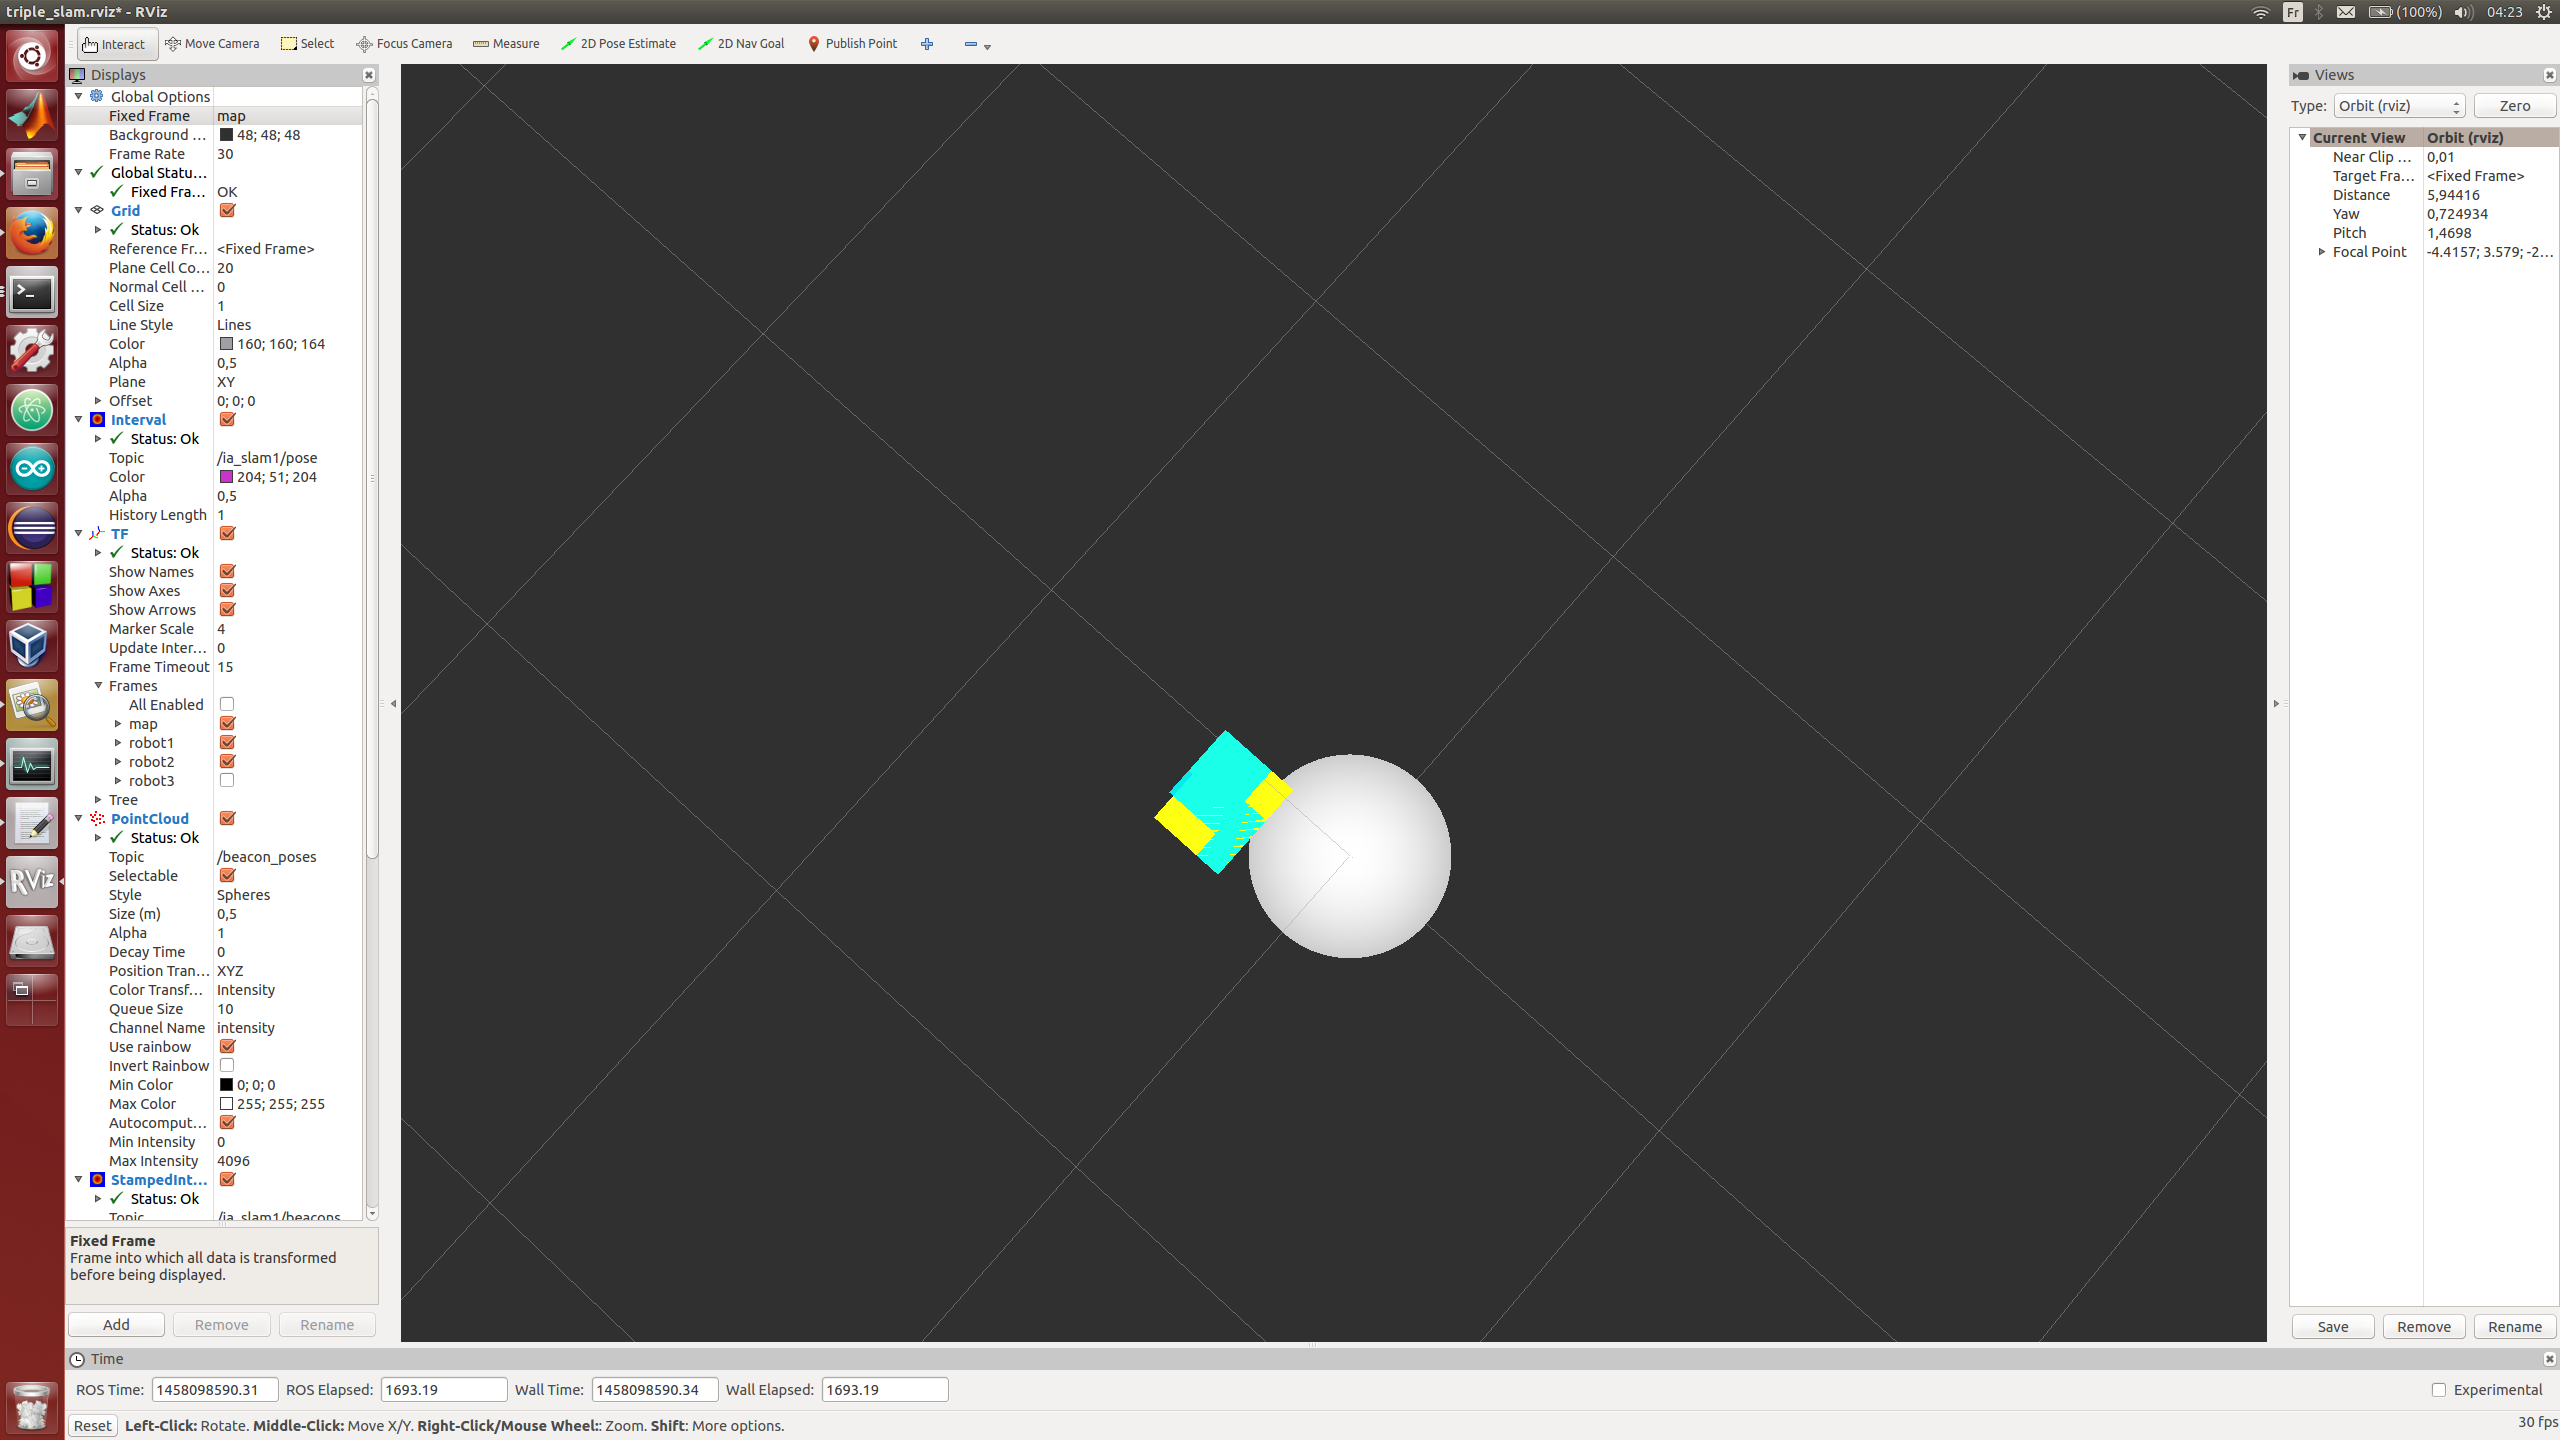
\includegraphics[trim={35cm 15cm 30cm 15cm},clip,scale=0.2,angle=0]{error.png}
\caption{Error on the beacon estimate.}
\label{fig:errorEst}
\end{figure}

The interval method is supposed to give a guaranteed results therefore the problem has to come from the implementation,either there is wrong data in the input,dela in communication is too important(see subsection~\ref{ssec:delaycompProb}), or the state equation used is wrong( but it is working for the robot alone).
By repeating the test it can be seen that the problem originates from the start of the test and there is wrong calculation on the pose estimate.